%==================================================
% This is for generating a standalone sprint 2 plan
%==================================================
\documentclass[a4paper, 11pt]{report}
\usepackage[T1]{fontenc}
\usepackage[utf8]{inputenc}
\usepackage[english]{babel}
\usepackage{graphicx} % support graphics
\usepackage{hyperref} % links in the document
\usepackage{float} % position of figures
\usepackage{paralist} % inline lists
\usepackage{verbatim} % multiline comments
\usepackage[table]{xcolor} % table row coloring
\usepackage{booktabs} % Professional tables
\usepackage{tabularx} % Simple column stretching
\usepackage{multirow} % Row spanning
\usepackage{wrapfig} % Wrap text around figures
\usepackage{array}
\usepackage{listings}
\usepackage{color}
\usepackage{textcomp}
\usepackage[style=treenoname,subentrycounter,numberedsection, 
        section=chapter, acronym]{glossaries}


\definecolor{listinggray}{gray}{0.9}
\definecolor{lbcolor}{rgb}{0.9,0.9,0.9}

\lstset{
    backgroundcolor=\color{lbcolor},
    tabsize=4,
    rulecolor=,
    language=C,
    basicstyle=\footnotesize,
    upquote=true,
    aboveskip={1.5\baselineskip},
    columns=fixed,
    showstringspaces=false,
    extendedchars=true,
    breaklines=true,
    prebreak = \raisebox{0ex}[0ex][0ex]{\ensuremath{\hookleftarrow}},
    frame=single,
    showtabs=false,
    showspaces=false,
    showstringspaces=false,
    identifierstyle=\ttfamily,
    keywordstyle=\color[rgb]{0,0,1},
    commentstyle=\color[rgb]{0.133,0.545,0.133},
    stringstyle=\color[rgb]{0.627,0.126,0.941},
}

% Configure links in pdfs
\hypersetup{
    bookmarksopen=false, % Hide bookmarks menu
    colorlinks=true, % Don't wrap links in colored boxes
}

\title{Introduction}
\author{Kpro group 9}
\date{\today}

\begin{document}
%\maketitle
%\tableofcontents
\makeglossaries
\newglossaryentry{wireshark}{name={Wireshark},
description={Program used to analyze packet data sent between network nodes}}

\newglossaryentry{python}{name={Python},
description={A programming language}}

\newglossaryentry{mac}{name={Mac},
description={A brand of personal computers}}

\newglossaryentry{linux}{name={Linux},
description={An operating system}}

\newglossaryentry{c}{name={C},
description={A programming language}}

\newglossaryentry{clang}{name={clang},
description={A compiler front-end for different \Gls{c} programming languages}}

\newglossaryentry{gcc}{name={gcc},
description={define this}}

\newglossaryentry{c++}{name={C++},
description={A programming language}}

\newglossaryentry{java}{name={Java},
description={A programming language}}

\newglossaryentry{lua}{name={Lua},
description={A programming language, often used for making \glspl{script}}}

\newglossaryentry{script}{name={script},
description = {A list of commands that are executed by a certain program, usually as an extension of the original functionality},
plural=scripts} 

\newglossaryentry{int}{name={int},
description={See \gls{integer}}}

\newglossaryentry{double}{name={double},
description={DEFINE}}

\newglossaryentry{integer}{name={integer},
description={define this},
plural=integers}

\newglossaryentry{char}{name={char},
description={define this},
plural=chars}

\newglossaryentry{float}{name={float},
description={define this},
plural=floats}

\newglossaryentry{pycparser}{name={pycparser},
description={A \Gls{c} \gls{parser} written in \Gls{python}}}

\newglossaryentry{ply}{name={ply},
description = {A \Gls{python} \gls{library} for creating \glspl{lexer} and \glspl{parser}}}

\newglossaryentry{parser}{name={parser},
description = {A program that receives input, checks it for correct syntax and builds a data structure representing the input},
plural=parsers}

\newglossaryentry{lexer}{name={lexer},
description = {A lexer is a program that converts a sequence of characters into a sequence of tokens},
plural=lexers}

\newglossaryentry{token}{name={token},
description = {A string of characters, categorized as a symbol according to a set of given rules},
plural=tokens}

\newglossaryentry{dissector}{name={dissector},
description = {Code that decodes \gls{packet} data and makes it readable by humans},
plural=dissectors}

\newglossaryentry{packet}{name={packet},
description = {Small block of data transmitted over a network},
plural=packets}

\newglossaryentry{utility}{name={utility},
description = {A small program that supports larger applications by doing certain tasks},
plural=utilities}

\newglossaryentry{library}{name={library},
description = {A collection of pre-written code for aiding programmers in the development process},
plural=libraries}

\newglossaryentry{ipc}{name={inter-process communication},
description = {The exchange of data that happens between \glspl{process}}}

\newglossaryentry{process}{name={process},
description = {A program running on a computer},
plural=processes}

\newglossaryentry{struct}{name={struct},
description = {Short for structure, it is a type that groups several \glspl{member} into a single \gls{object}},
plural=structs}

\newglossaryentry{member}{name={member},
description = {define this},
plural=members}

\newglossaryentry{binary}{name={binary},
description = {Two base arithmetic using the digits 0 and 1}}

\newglossaryentry{binary file}{name={binary file},
description = {A computer-readable file stored in \gls{binary} format}}

\newglossaryentry{nested struct}{name={nested struct},
description = {A \gls{struct} within another \gls{struct}},
plural={nested structs}}

\newglossaryentry{sparc}{name={SPARC},
description={A microprocessor architecture based on reduced instruction set computing}}

\newglossaryentry{version control system}{name={version control system},
description = {A system that ensures consistency of files when several people are collaborating on them},
plural={version control systems}}

\newglossaryentry{scrum}{name={Scrum},
description={A \gls{software development methodology}}}

\newglossaryentry{software development methodology}{name={software development methodology},
description={A framework used to structure, plan and control a development process},
plural={software development methodologies}}

\newglossaryentry{branch}{name={branch},
description={define this},
plural=branches}

\newglossaryentry{distributed repository model}{name={distributed repository model},
description={A distributed approach to a \gls{version control system}},
plural={distributed repository models}}

\newglossaryentry{markup language}{name={markup language},
description={A language for specifying the processing, definition and presentation of text}}

\newglossaryentry{capture file}{name={capture file},
description={A file containing the data that is captured from network or IPC traffic},
plural={capture files}}

\newglossaryentry{ascii}{name={ASCII},
description={A character encoding scheme}}

\newglossaryentry{character encoding scheme}{name={character encoding scheme},
description={A system that maps characters to something else, write more }}

\newglossaryentry{hexadecimal}{name={hexadecimal},
description={A number system where sixteen is the base}}

\newglossaryentry{hex dump}{name={hex dump},
description={A \gls{hexadecimal} view of computer data},
plural={hex dumps}}

\newglossaryentry{pcap-file}{name={pcap-file},
description={See \gls{capture file}},
plural={pcap-files}}

\newglossaryentry{protocol}{name={protocol},
description = {A system of rules for exchanging messages between machines},
plural=protocols}

\newglossaryentry{link-layer}{name={link-layer},
description = {The \gls{protocol} layer that is responsible for transferring data between two nodes}}

\newglossaryentry{repository}{name={repository},
description = {A central storage area where data is kept and maintained},
plural=repositories}

\newglossaryentry{Sun RPC}{name={Sun RPC},
description={The Unix equivalent of Remote Procedure Call}}

\newglossaryentry{corba}{name={CORBA},
description={This is an acronym}}

\newglossaryentry{asn1}{name={ASN.1},
description={This is an acronym}}

\newglossaryentry{makefile}{name={makefile},
description={A file that helps the make utility in the creation of executables from source code},
plural=makefiles}

\newglossaryentry{post-dissector}{name={post-dissector},
description = {define this},
plural=post-dissectors}

\newglossaryentry{boolean}{name={boolean},
description={A data type that represents logical truth, it has the value True or False},
plural=booleans}

\newglossaryentry{string}{name={string},
description={define this},
plural=strings}

\newglossaryentry{garbage collection}{name={garbage collection},
description={define this}}

\newglossaryentry{closure}{name={closure},
description={define this},
plural=closures}

\newglossaryentry{object}{name={object},
description = {define this},
plural=objects}

\newglossaryentry{C99}{name={C99},
description={define this}}

\newglossaryentry{GCC-XML}{name={GCC-XML},
description={define this}}

\newglossaryentry{xml}{name={xml},
description={A \gls{markup language}}}

\newglossaryentry{Objective-C++}{name={Objective-C++},
description={A programming language}}

\newglossaryentry{Objective-C}{name={Objective-C},
description={A programming language}}

\newglossaryentry{AST}{name={abstract syntax tree},
description={A tree represention of a compiled program}}

\newglossaryentry{data serialization}{name={data serialization},
description={define this}}

\newglossaryentry{perl}{name={perl},
description={A programming language}}

\newglossaryentry{php}{name={php},
description={A scripting language}}

\newglossaryentry{Ruby}{name={Ruby},
description={A programming language}}

\newglossaryentry{Javascript}{name={Javascript},
description={A scripting language}}

\newglossaryentry{Eclipse}{name={Eclipse},
description={An application aiding computer programmers in software development}}

\newglossaryentry{header}{name={header},
description={define this},
plural=headers}

\newglossaryentry{enumerated named value}{name={enumerated named value},
description={define this},
plural={enumerated named values}}

\newglossaryentry{union}{name={union},
description={define this},
plural=unions}

\newglossaryentry{array}{name={array},
description={A data type that can hold a collection of elements},
plural=arrays}

\newglossaryentry{preprocessor}{name={preprocessor},
description={Define this},
plural=preprocessors}

\newglossaryentry{include}{name={\#include},
description={A \Gls{c} directive that includes other \gls{header} files to the current file}}

\newglossaryentry{if}{name={\#if},
description={A \Gls{c} directive that executes a statement if a given expression holds true }}

\newglossaryentry{ifdef}{name={\#ifdef},
description={A \Gls{c} directive that checks if a given token has been defined}}

\newglossaryentry{define}{name={\#define},
description={A \Gls{c} directive that can be used to define a constant or create a macro}}

\newglossaryentry{trailers}{name={trailers},
description={define this}}

\newglossaryentry{bit string}{name={bit string},
description={define this}
plural={bit strings}}

\newglossaryentry{endian}{name={endian},
description={See \gls{endianness}},
plural=endians}

\newglossaryentry{endianness}{name={endianness},
description={Refers to the ordering of bytes in a word. A big-endian machine stores the most significant byte first, and a little-endian the least significant.}}

\newglossaryentry{batch mode}{name={batch mode},
description={define this}}

\newglossaryentry{batch processing}{name={batch processing},
description={See \gls{batch mode}}}

\newglossaryentry{x86}{name={x86},
description={The instruction set architecture used by Intel processors}}

\newglossaryentry{Windows}{name={Windows},
description={An operating system by Microsoft}}

\newglossaryentry{Solaris}{name={Solaris},
description={An operating system by Sun Microsystems}}

\newglossaryentry{x86-64}{name={x86-64},
description={An extension of the \gls{x86} instruction set that is compatible with 64-bit processors}}

\newglossaryentry{Field}{name={Field},
description={define this}}

\newglossaryentry{argparse}{name={argparse},
description={define this}}

\newglossaryentry{enum}{name={enum},
description={See /gls{enumerated named value}},
plural=enums}

\newglossaryentry{wildcard}{name={wildcard},
description={define this}}

\newglossaryentry{x-86}{name={x-86},
description={define this}}



\newacronym{ntnu}{NTNU}{Norwegian University of Technology and Science}
%=====================
\chapter{Introduction}
%=====================

This chapter is a technical introduction to our project.
It gives a concise explanation of the most important terms used in the report.

The first section briefly explains \Gls{wireshark}, \glspl{dissector} and how \glspl{dissector} are used in \Gls{wireshark}.
The connection between \Gls{wireshark} and the \Gls{lua} \glspl{struct} \gls{protocol} is also explained.

The second section describes how the \Gls{lua} code works and how it is generated by our \gls{utility}.

%---------------------------------
\section{Wireshark and Dissectors}
%---------------------------------
This section gives a brief introduction to \Gls{wireshark} and \glspl{dissector}.
The first part describes what \Gls{wireshark} is and what it can be used for.
The second part explains exactly what a \gls{dissector} is, and how a \gls{dissector} can be used to extend \Gls{wireshark}.

\subsection{Wireshark}
%---------------------
\Gls{wireshark} is a program used to analyze network traffic. A common usage scenario is when a person wants to troubleshoot network problems or
look at the internal workings of a network \gls{protocol}. An important feature of \Gls{wireshark} is the ability to capture and display a live stream of \glspl{packet} sent through the network. 
A user could, for example, see exactly what happens when he opens up a website. \Gls{wireshark} will then display all the messages
sent between his computer and the web server. It is also possible to filter and search on given \gls{packet} attributes, which facilitates the debugging \gls{process}.

In \autoref{fig:introshark}, you can see a view of \Gls{wireshark}.
This specific example shows a capture file with four messages, or \glspl{packet}, sent between internal \glspl{process}, in other words
it is a view of messages sent by inter-\gls{process} communication. Each of the \glspl{packet} contain one \Gls{c} \gls{struct}.
To be able to display the contents of the \Gls{c} \gls{struct}, \Gls{wireshark} must be extended. 
This can be accomplished by writing a \gls{dissector} for the \Gls{c} \gls{struct}.

\Gls{wireshark} \glspl{dissector} can be written in either \Gls{c} or \Gls{lua}, and in our \gls{utility} they are written in \Gls{lua}.
The difference between \Gls{c} and \Gls{lua} \glspl{dissector},
and the reason we used \Gls{lua} is elaborated on in the 
preliminary study in \autoref{cha:prestudy}.
Dissectors, in general, are explained more in detail below.

\begin{figure}[htb]
	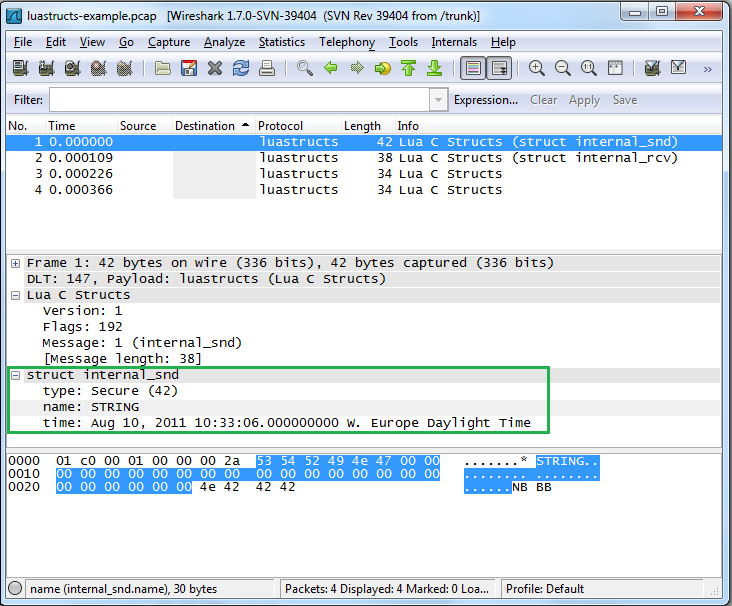
\includegraphics[width=\textwidth]{./img/wireshark_example.png}
	\caption{Wireshark Screenshot\label{fig:introshark}}
\end{figure}

\subsection{Dissectors}
%----------------------
In short, a \gls{dissector} is a piece of code, run on a blob of data, which can dissect the
data and display it in a readable format in \Gls{wireshark}, instead of the \gls{binary} representation.

\autoref{fig:introshark} displays four \glspl{packet}, with \gls{packet} number 1 highlighted.
The content of the \gls{packet} is a \Gls{c} \gls{struct} with two \glspl{member}, name and time, and it is displayed inside the green box.
The \Gls{c} code for the \gls{struct} is shown in \autoref{structexample}.
The \gls{dissector} takes the \Gls{c} \gls{struct}, decodes its \gls{binary} representation and makes it readable by humans.
Without a \gls{dissector}, \Gls{wireshark} would just display the \gls{struct} and \gls{struct} \glspl{member} as a \gls{binary} blob.

All the \glspl{packet} containing \Gls{c} \glspl{struct} belong to the \gls{protocol} called luastructs.
When opening a capture file in \Gls{wireshark} , this \gls{protocol} maps the id of the messages to the correct \gls{dissector},
and calls them.

\lstset{language=C,caption={Example C Struct},label=structexample}
\lstinputlisting[language=C]{./code/struct.h}

%------------------------------------------------------------------
\section{From \Gls{struct} definition to \Gls{lua} \Gls{dissector}}
%------------------------------------------------------------------
This section explains what happens under the hood of a \Gls{lua} \gls{dissector}.

\begin{comment}
, and how they can be built by our \gls{utility}.
The first part explains what happens under the hood of a \Gls{lua} \gls{dissector}, while 
the second part is a very brief explanation of how CSjark builds such \glspl{dissector}.
\end{comment}

\subsection{\Gls{lua} \Glspl{dissector}}
%---------------------------------------
\autoref{luaexample1} shows what the code for the \Gls{lua} \gls{dissector}, displayed in \gls{packet} 1 in \autoref{fig:introshark}, looks like.
The Proto variable defines a new \gls{protocol}. In this example, a \gls{dissector} for the internal\_snd \gls{struct}, called internal\_snd, is created. 
The different fields of the \gls{struct} are created as instances of ProtoField, and put in Protocol.fields.
For example, the ''name'' variable is a \gls{string} in \Gls{c}, and as such it is created as a ProtoField.\gls{string} with the 
name ''name''.

The \gls{protocol} \gls{dissector} method is the method that does the actual dissecting.
A subtree for the \gls{dissector} is created, and the description of the \gls{dissector} is appended to the information column.
All the ProtoFields are added to the subtree. Here you can see that the type, name and time fields are added to the subtree for the internal\_snd \gls{dissector}.
The buffer size allocated to the fields is the size of the \glspl{member} in \Gls{c}.

In the last line the \gls{dissector} is added to the \gls{dissector} table as a subdissector for the luastructs \gls{protocol}.
When running a capture file, where the internal\_snd \gls{struct} is being sent to another \gls{process}, it is possible to see the exact contents of the \gls{struct}, as the example screenshot of \Gls{wireshark} shows.

\newpage
\lstset{language=C,caption={Example Lua File},label=luaexample1}
\lstinputlisting[language=C]{./code/luaexample1.lua}

\begin{comment}
\subsection{CSjark - Automated generation of \Gls{lua} \glspl{dissector}}
CSjark is a \Gls{python} \gls{utility} that can automatically generate a \Gls{lua} \gls{dissector} for 
any valid \Gls{c} \gls{header} file. It also supports user configuration from files in a specific format.
The \Gls{c} file, in addition to any suitable configuration file, is inputted into a command line interface.
The \Gls{c} file is then sent to the \Gls{c} preprocessor, where \Gls{c} directives are evaluated before the parsing.
The \gls{parser} creates an abstract syntax tree from the input.
CSjark traverses the abstract syntax tree and finds all the \gls{struct} definitions.
For every \gls{struct} that is found, a \gls{dissector} is generated and written to file.
\end{comment}


\end{document}

